\chapter{Preface: The Ahuora Digital Twin Platform}


%This chapter has been included based on feedback from the mid-progress report that the marker did not understand the context of the project.
\textit{ Unlike many other projects, this project is part of a larger, multi-disciplinary project. Occasionally, work has focused on broader platform development rather than solely on this sub-project. Additionally, some work involves research for future implementations that cannot be completed with the platform's current capabilities. This chapter provides an overview of the Ahuora Digital Twin Platform, to provide context for the rest of the report.}

\section{Background}

`Project Ahuora' is a Ministry of Business, Innovation and Employment (MBIE) funded project that aims to decarbonise the process heat sector.
By decarbonising, New Zealands' greenhouse gas emissions will be reduced. Cost savings from reduced energy consumption are anticipated, along with increased energy independence.
This is a multi-disciplinary project that involves researchers from the University of Waikato, University of Auckland, Massey University,
and other global universities. Chemical Engineers bring understanding of the chemical processes that are used in industry. Electrical Engineers bring understanding of the grid system
and how to integrate renewable energy sources. Mechanical engineers bring understanding of how to design and build more efficient systems. Software Engineers bring understanding of how to
model, simulate, and monitor complex systems.

A key objective is to develop a digital twin platform for the chemical processing industry. This platform will allow New Zealand factory operators to model their processes, simulate different scenarios, and monitor their processes in real-time.
This will enable factory operators to make data-driven and scientifically backed decisions on how to improve their processes. A digital twin can recognise where the factory is underperforming, suggest real-time improvements, and help plain future investments.

\section{The Ahuora Simulation Platform}

A key deliverable of the Ahuora project to date is the Ahuora Simulation Platform. This is a web-based platform that allows users to model a factory or other energy system, and simulate its performance. The platform is based on the IDAES Process Systems Engineering Framework, which is a Python library that provides tools for modelling and simulating chemical processes.

Currently, the platform can model a factory at a single point in time. The user specifies the properties of the factory, such as the flow rates of different materials, the temperature and pressure of different streams, and the efficiency of different unit operations. The platform then simulates the factory and provides the user with a report on the factory's performance.

\subsection{Flowsheet Interface}


\begin{figure}
    \centering
    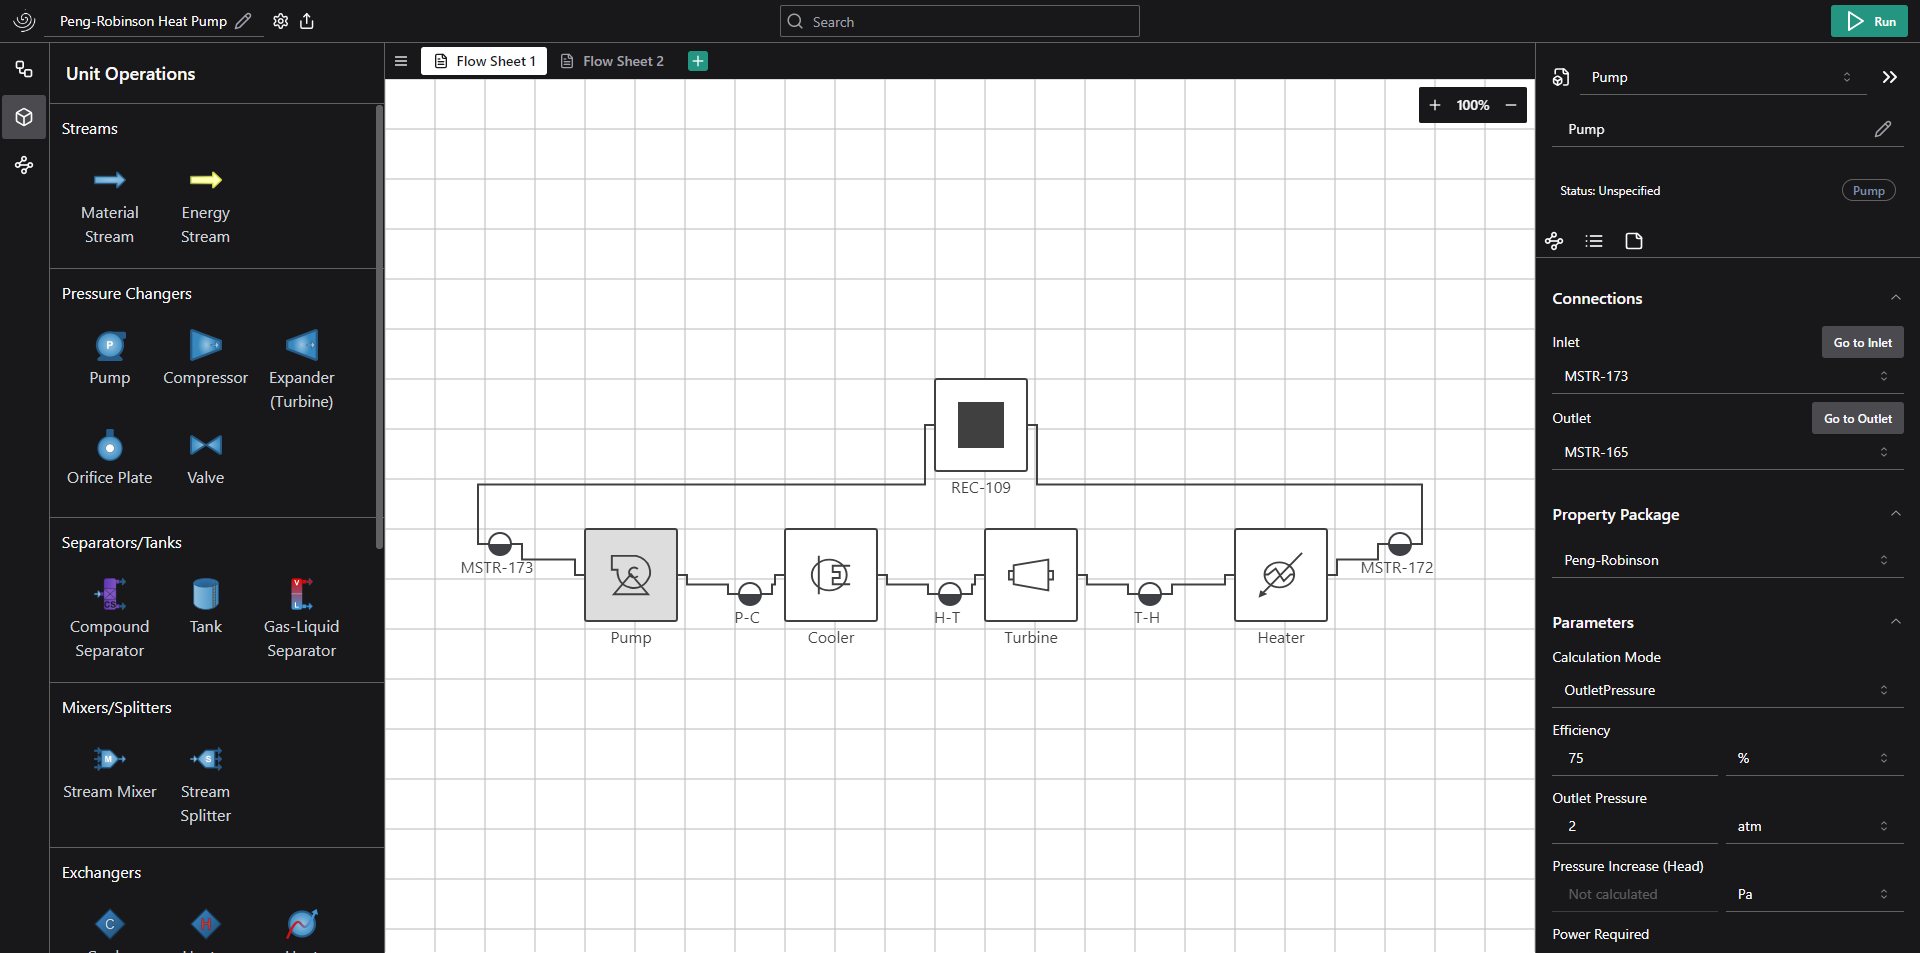
\includegraphics[width=\textwidth]{platform_screenshot.png}
    \caption{Example Flowsheet in the Ahuora Simulation Platform}
    \label{fig:platform}
\end{figure}

\Cref{fig:platform} shows a screenshot of the Ahuora Simulation Platform, as at August 2024. The user interface is divided into three main sections. The left-hand panel shows a list of unit operations from a factory, including pumps, heaters, heat exchangers, reactors, and material streams. The user can drag and drop these unit operations onto the canvas in the centre of the screen. The user can then connect the unit operations together to create a process flow diagram. The right-hand panel shows the properties of the selected unit operation, such as the flow rate of the material stream, the temperature and pressure of the stream, and the efficiency of the unit operation. The user can edit these properties to simulate different scenarios.

The displayed flowsheet shows a simple heat pump cycle. The block on the top is a ``recycle", specifying that the output of the cooler is fed back into the pump. A more complex flowsheet would replace the cooler and heater with heat exchangers, which exchange heat with their environment, but this provides a simple example.

\subsection{Online Integration}

\begin{figure}
    \centering
    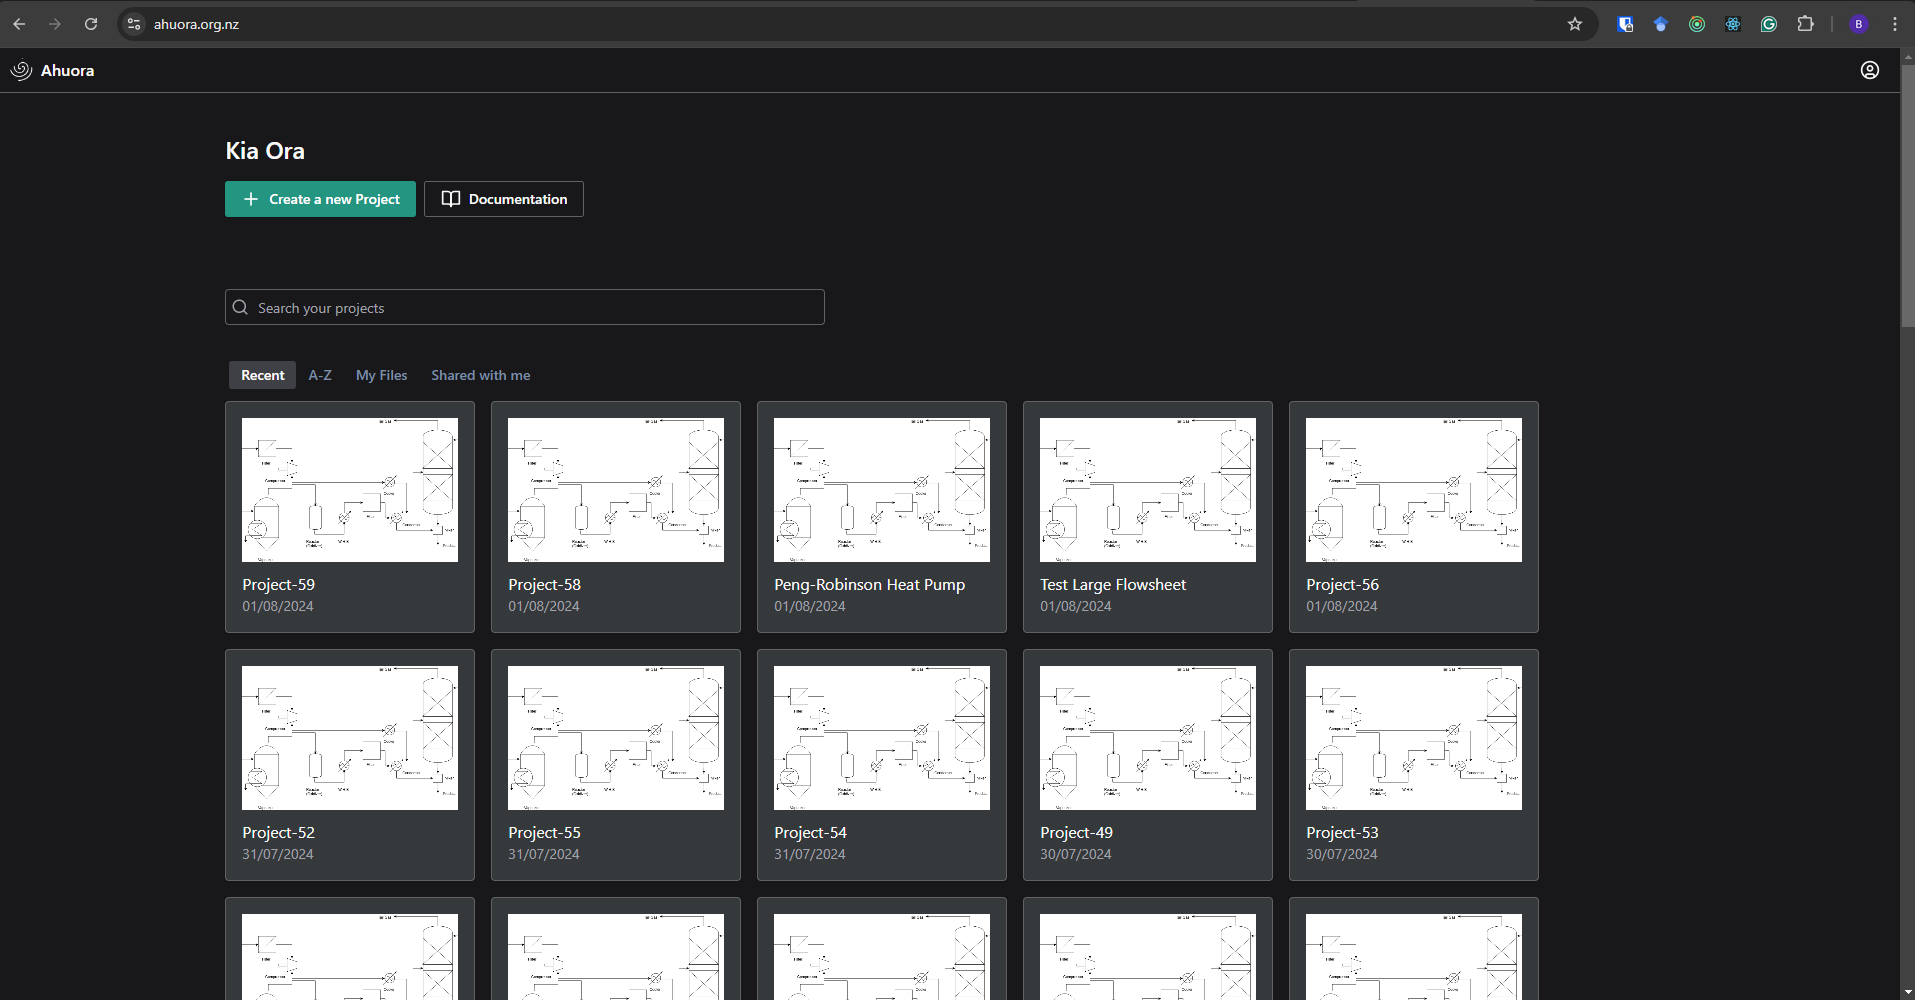
\includegraphics[width=\textwidth]{platform_homepage.png}
    \caption{Homepage of The Ahuora Simulation Platform}
    \label{fig:homepage}
\end{figure}

The Ahuora Simulation Platform is designed as a web-based multi-user platform. This offloads processing and data storage to the server, allowing users to access the platform from any device with a web browser. Simulation can be very computationally expensive, particuarly in advanced models, so this is a key feature. It enables simulation to be run in parallel on powerful servers, and allows the platform to be used in industry without requiring significant upfront investment in hardware. In future, this will also enable the platform to be used for real-time collaboration between multiple users. Its API allows it to be integrated with other software, enabling enhanced functionality, real-time updates, and broader interactions.

The home page of the platform, shown in \cref{fig:homepage}, provides a list of saved simulations, and allows the user to create a new simulation. This is not publicly acessible, as the platform is still in development, and user account functionality is not yet complete.

\section{The Ahuora Digital Twin Platform}

There are a number of objectives that Ahuora is working towards including in the platform. These include:

\begin{itemize}
    \item Steady-state Process Simulation: This is the current state of the platform. However, it can be improved by adding support for:
          \begin{itemize}
              \item More unit operations, defined from first principles equations
              \item Custom unit operations
              \item Unit operations defined from data (Machine Learning \& Hybrid Modelling)
              \item More property packages (enabling accurate simulation of a wider range of chemical processes)
              \item Support for more advanced mathematical constraints
          \end{itemize}
    \item Advanced analysis techniques: This includes:
          \begin{itemize}
              \item P-Graph Analysis, generating and comparing alternative process structures
              \item Pinch Analysis, to identify the theorical minimum energy consumption of a process
              \item Heat Exchanger Network analysis, to identify opportunities for heat recovery in individual processes
              \item Utility System Analysis, to identify opportunities for energy savings on a plant-wide scale
          \end{itemize}
    \item Process Variable Optimisation: Calculating the optimal operating conditions (temperatures, pressures, flow rates, power utilisation) for a given process
    \item Dynamic simulation, to model the factory over time, so that the effect of changes on can be predicted
    \item Process Scheduling, to optimise the factory's resources across tasks
    \item Live Data Processing, to:
          \begin{itemize}
              \item simulate plant conditions in real-time, for performance monitoring and diagnostics
              \item update the simulation based on real-world changes, e.g fouling or equipment degradation
          \end{itemize}
    \item Process Control - adjusting the physical process plant based on the simulation to maintain desired operating conditions
    \item Reporting functionality, such as Process \& Instrumentation diagrams.
\end{itemize}

For clarity in this report, the term ``Ahuora Digital Twin Platform" will refer to the complete solution, keeping in mind all these future objectives. The term ``Ahuora Simulation Platform" will refer to the current state of the platform, which is based on steady-state simulation, and does not yet support the features required for a Digital Twin.

\section{The Role of This Project}

This project contributes to a number of these objectives, utilising the Ahuora Simulation Platform as a base, updating it to work with real-time data, and developing a standardised framework for integrating real-time sensor data into the platform. This provides the groundwork to support the advanced analysis techniques, process variable optimisation, dynamic simulation, and live data processing that are required for a Digital Twin.
